\chapter{Einleitung}
\label{ch:intro}

\section{Motivation}
\label{sec:intro:motivation}
Viele Unternehmen verfügen über sensible Informationen, sei es zum Beispiel Versicherungen oder Krankenhäuser. Sensibel Informationen können dabei Telefonnummern oder auch Namen  und Adressen sein.
Diese Informationen werden auf gesicherten Servern gelagert, auf welche nur bestimmte Personen Berechtigungen haben.
Diese Personen verfügen über Profile, die ihnen diese Berechtigungen verfügen.
Jedoch kann es passieren, dass solche Profile gestohlen oder Personen gegeben werden, welche diese nicht haben sollten.
Berechtigungstrukturen sollen genau diese Szenarien verhindern.
Wird aber eine Berechtigungstruktur lange genutzt und werden nicht alle Richtlinien und Normen eingehalten, so wird diese im laufe der Zeit unsicherer und unübersichtlicher.
Das hat zur Folge, dass das Risiko, dass die sensitiven Informationen in nicht autorisierten Hände kommen, steigt.
Dadurch können sogenannte "`Super Accounts"' entstehen.
"`Super Accounts"' verfügen über zu viele, bis zu allen Berechtigungen im System.
Sollte diese Person durch einen Angriff diesen "`Super Account"' verlieren, wäre die gesamte Struktur kompromitiert.
Dasselbe ist der Fall, wenn ein Mitarbeiter mit einem solchen Account dem Unternehmen schaden will.

\begin{figure}[h!]
 \centering
 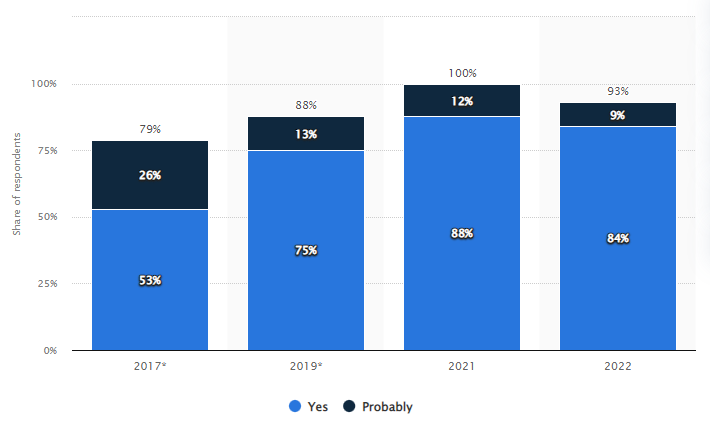
\includegraphics[width=1\textwidth]{gfx/Picture/Cyber_Crime.PNG}
 \caption{Eine Umfrage von Deutschen Unternehmen, die von Daten Diebstahl, Espionage oder Sabotage betroffen waren.\cite{Stat22}}
 \label{fig:Crime}
\end{figure}

Wie man in der Grafik (\ref{fig:Crime}) erkennen kann, waren 88\% der befragten Unternehmen in Deutschland von Datendiebstahl, Espionage oder Sabotage in 2021 betroffen.
In 2022 liegt die Zahl bei 84\%.
Wobei man berücksichtigen muss, dass diese Befragung zwischen Januar and März statt gefunden und dies daher nur das erste Quartal von 2022 abdeckt.
Aufgrund dessen, dass solche Angriffe wahrscheinlich sind, darf es keine "`Super Accounts"' geben, da diese ansonsten in solchen Angriffen als Schwachstelle ausgenutzt werden könnten.
Genauso müssen die Strukturen übersichtlich sein, damit bei einer Überprüfung es keine Probleme darstellt, festzustellen, welcher Nutzer welche Berechtigungen hat.
Wenn dies nicht der Fall ist, kann es passieren, dass die jeweiligen Nutzern zu viele Berechtigungen haben und dies wäre wieder ein Problem bei Espionage oder Sabotage.
Um dies zu erreichen gibt es verschiedene Methoden und Konzepte, die die Berechtigungsstrukturen sicher und übersichtlich gestalten.

%
% Section: Ziele
%
\section{Ziel der Arbeit}
\label{sec:intro:goal}
Diese Arbeit ist eine Vergleicharbeit bei der verschiedene Konzepte verglichen werden.
Dabei wird auf die folgende Fragestellung in dieser Arbeit eingegangen, \textit{inwieweit man bestehende Berechtigungsstrukturen im Hostbereich verändern und optimieren kann}.
Dazu gibt des drei Unterfragen, welche verwendet werden, um die Problemstellung systematisch zu beantworten.

\begin{itemize}
  \item \textit{Welche Konzepte werden derzeit für Berechtigungstrukturen verwendet, um diese sicher und übersichtlich zu gestalten?}
  \item \textit{Wie unterscheiden sich die verschiedenen Konzepte?}
  \item \textit{Womit kann man die verschiedenen Konzepte vergleichen?}
\end{itemize}

Die erste Unterfrage wird durch eine Recherche mit verschiedenen Arbeiten im Bereich der Berechtigungstruktur beantwort.
Dies soll einen Überblick zum Stand der Technik geben.
Anschließend wurden mehrere Beafragung durch geführt, um die bestehenden Konzepten nach den Wünschen der Befragten anzupassen.
Darauf basierend werden die bestehenden Methoden geranked und verglichen.
Dies beantwortet die zweite Unterfrage mittels des erstellten Vergleiches.
\newline
Um die dritte Frage zu beantworten wird ein Schema verwendet, welches als eine Hilfestellung zur Konzeptauswahl dienen wird.
Zum Schluss wird eine alternative zum bestehenden System vorgestellt.
Dies ist die Arbeit in visueller Form.

\begin{figure}[h!]
 \centering
 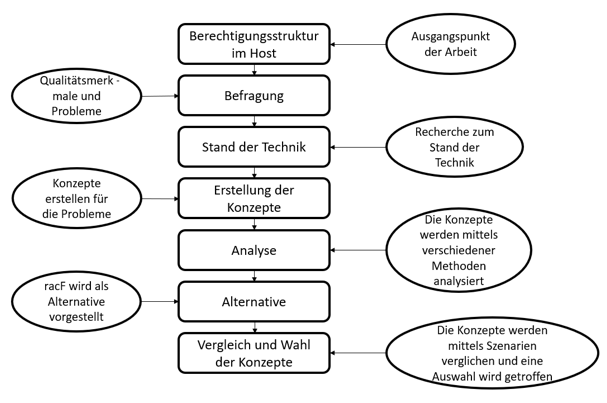
\includegraphics[width=0.75\textwidth]{gfx/Picture/Vorgehen.PNG}
 \caption{Aufbau der Arbeit}
 \label{fig:vorgehen}
\end{figure}